\chapter{Design Solution}
\label{chap:design}
In this project we aim to create an LSM-structured implementation of R-trees, which in turn will be write-optimized. To be able to handle a high workload of write operations without compromising query performance, a bulk-insertion technique such as GBI\cite{GBI} or Seeded Clustering\cite{SeededClustering} will be used to make sure that the index structure is not degraded too much. In addition, the use of such techniques will hopefully also generate better storage utilisation which is needed to avoid unnecessary search operations. We have chosen to call the design solution a \emph{Rectangle-Structured Merge Tree} or RSM-Tree.

\section{Overview}
In order to implement an R-tree index while having a LSM-tree structure, there are some important design choices that need to be evaluated. The first is the ordering of the data, as R-trees are used for multidimensional data, while LSM-trees are not. In order to do this, the use of space-filling curves are needed, such as Z-order curve or Hilbert curve. In this design solution, the main ordering technique will be the Z-order curve, but both curves might be tested in a future implementation. Another important aspect is how to merge the data from the upper levels to the lower levels. To do this we have chosen to use bulk-insertion methods which looks at loading smaller R-trees into larger ones. By doing this, the costly operation of creating R-trees from scratch will not be needed with every merge.\newline

\noindent
Lastly, the choice of merge policies is important. Inspired from Dostoevsky\cite{Dostoevsky}, we hope to try different combinations of tiering and leveling policies as explained in Section \ref{Dostoevsky}. In the first design solution, \emph{Lazy Leveling} will be used.  

\section{Structure}
The general structure of the RSM-tree is presented in Figure \ref{fig:RSMTree}. The in-memory component $C_0$ stores each data object in their own MBR, given as $A, B, ..., F$. These are sequentially ordered by the chosen space-filling curve. This is done because it is crucial that the items are sequentially ordered when performing search operations in LSM-trees. In addition to this, a sequential structure is beneficial when merging the data to the lower levels, as will be further explained in Section \ref{sect:RSM-Merging}. In the second level $C_1$, the MBRs will be merged together to create R-trees from scratch, given as $R_2, R_3, R_4, R_5$. The lowest level $C_2$, is structured as the main R-tree, where trees from $C_1$ will be bulk-inserted into the correct positions in the main R-tree.  
\begin{figure}[ht]
     \centering
     \begin{subfigure}{0.45\textwidth}
         \centering
         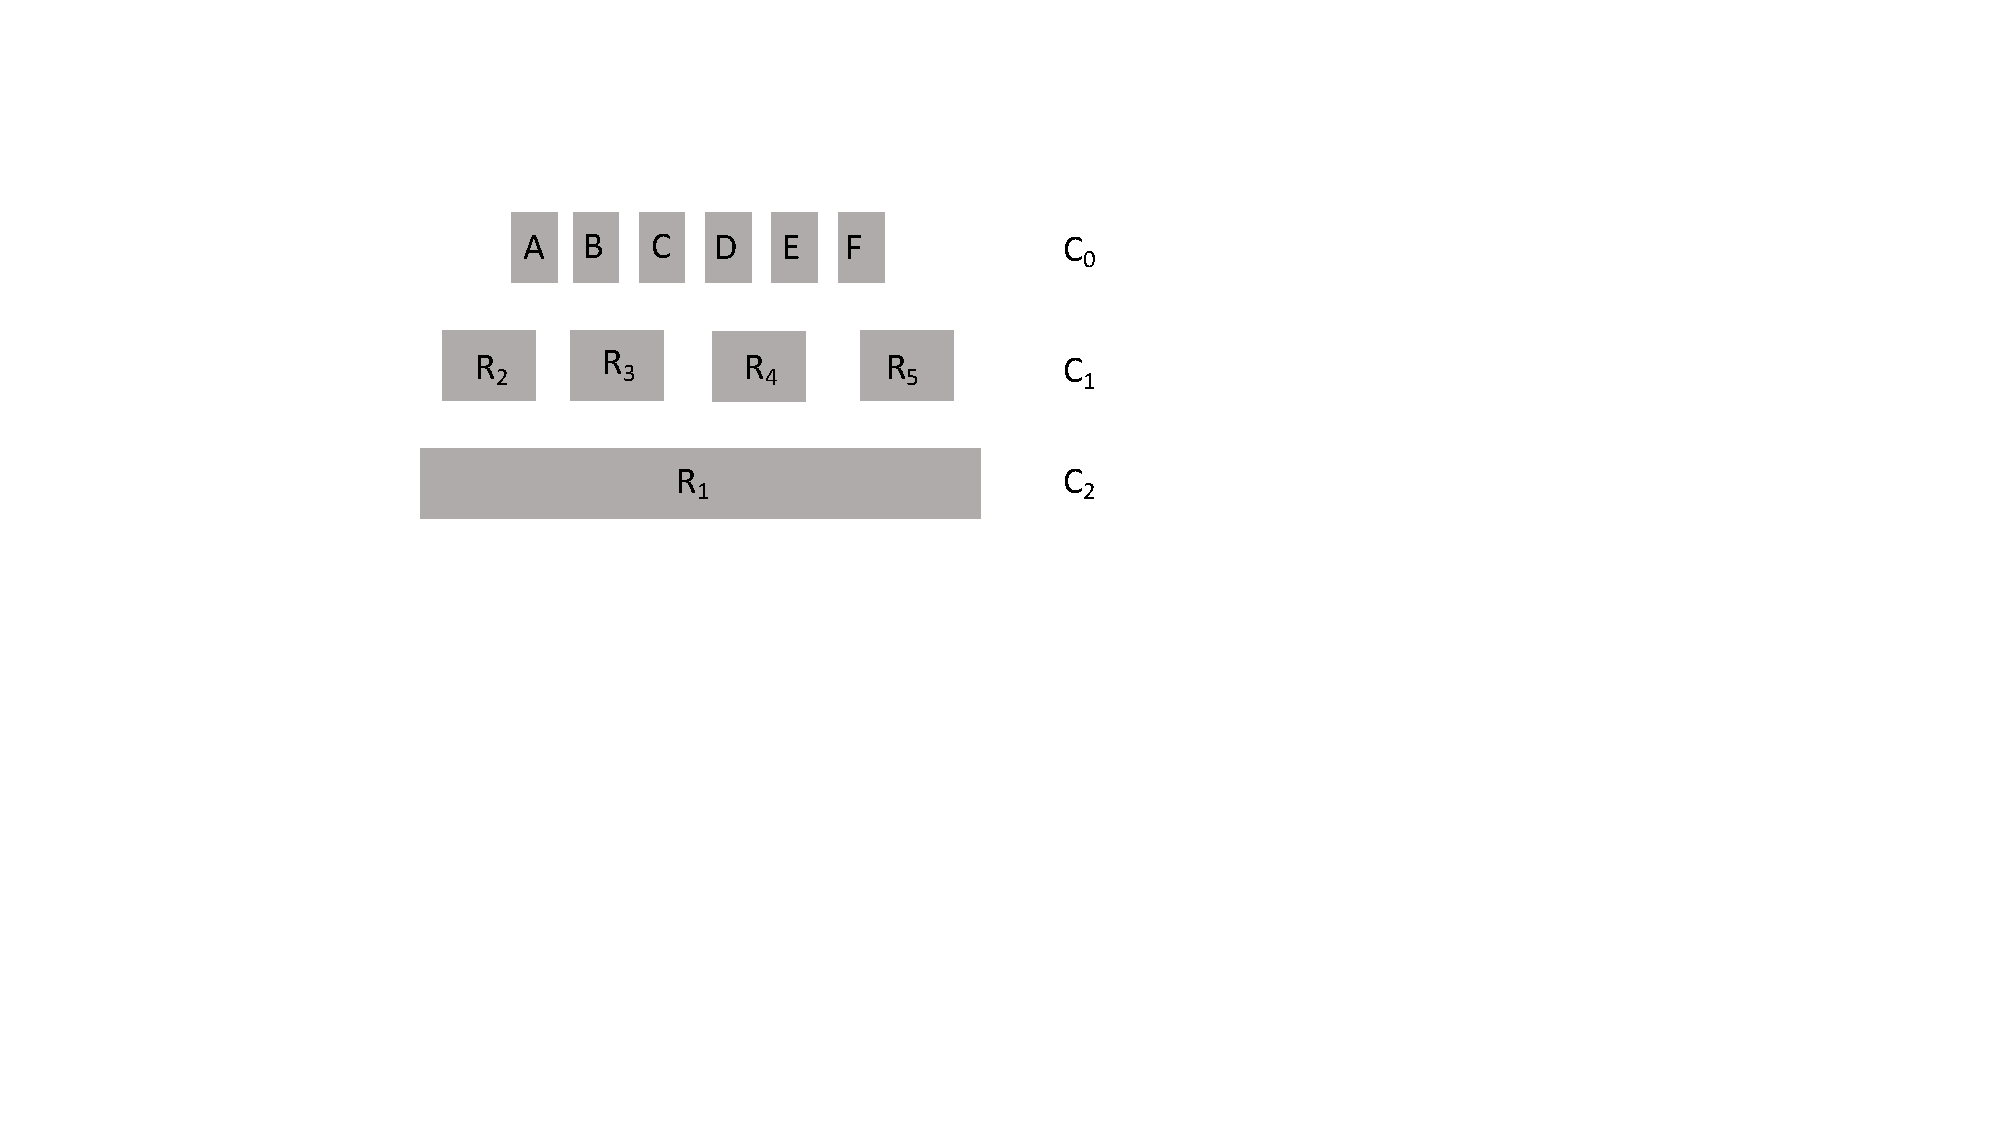
\includegraphics[width=\textwidth]{figures/RSMTree.pdf}
         \caption{RSM-Tree index structure}
     \end{subfigure}
     \hfill
     \begin{subfigure}{0.45\textwidth}
         \centering
         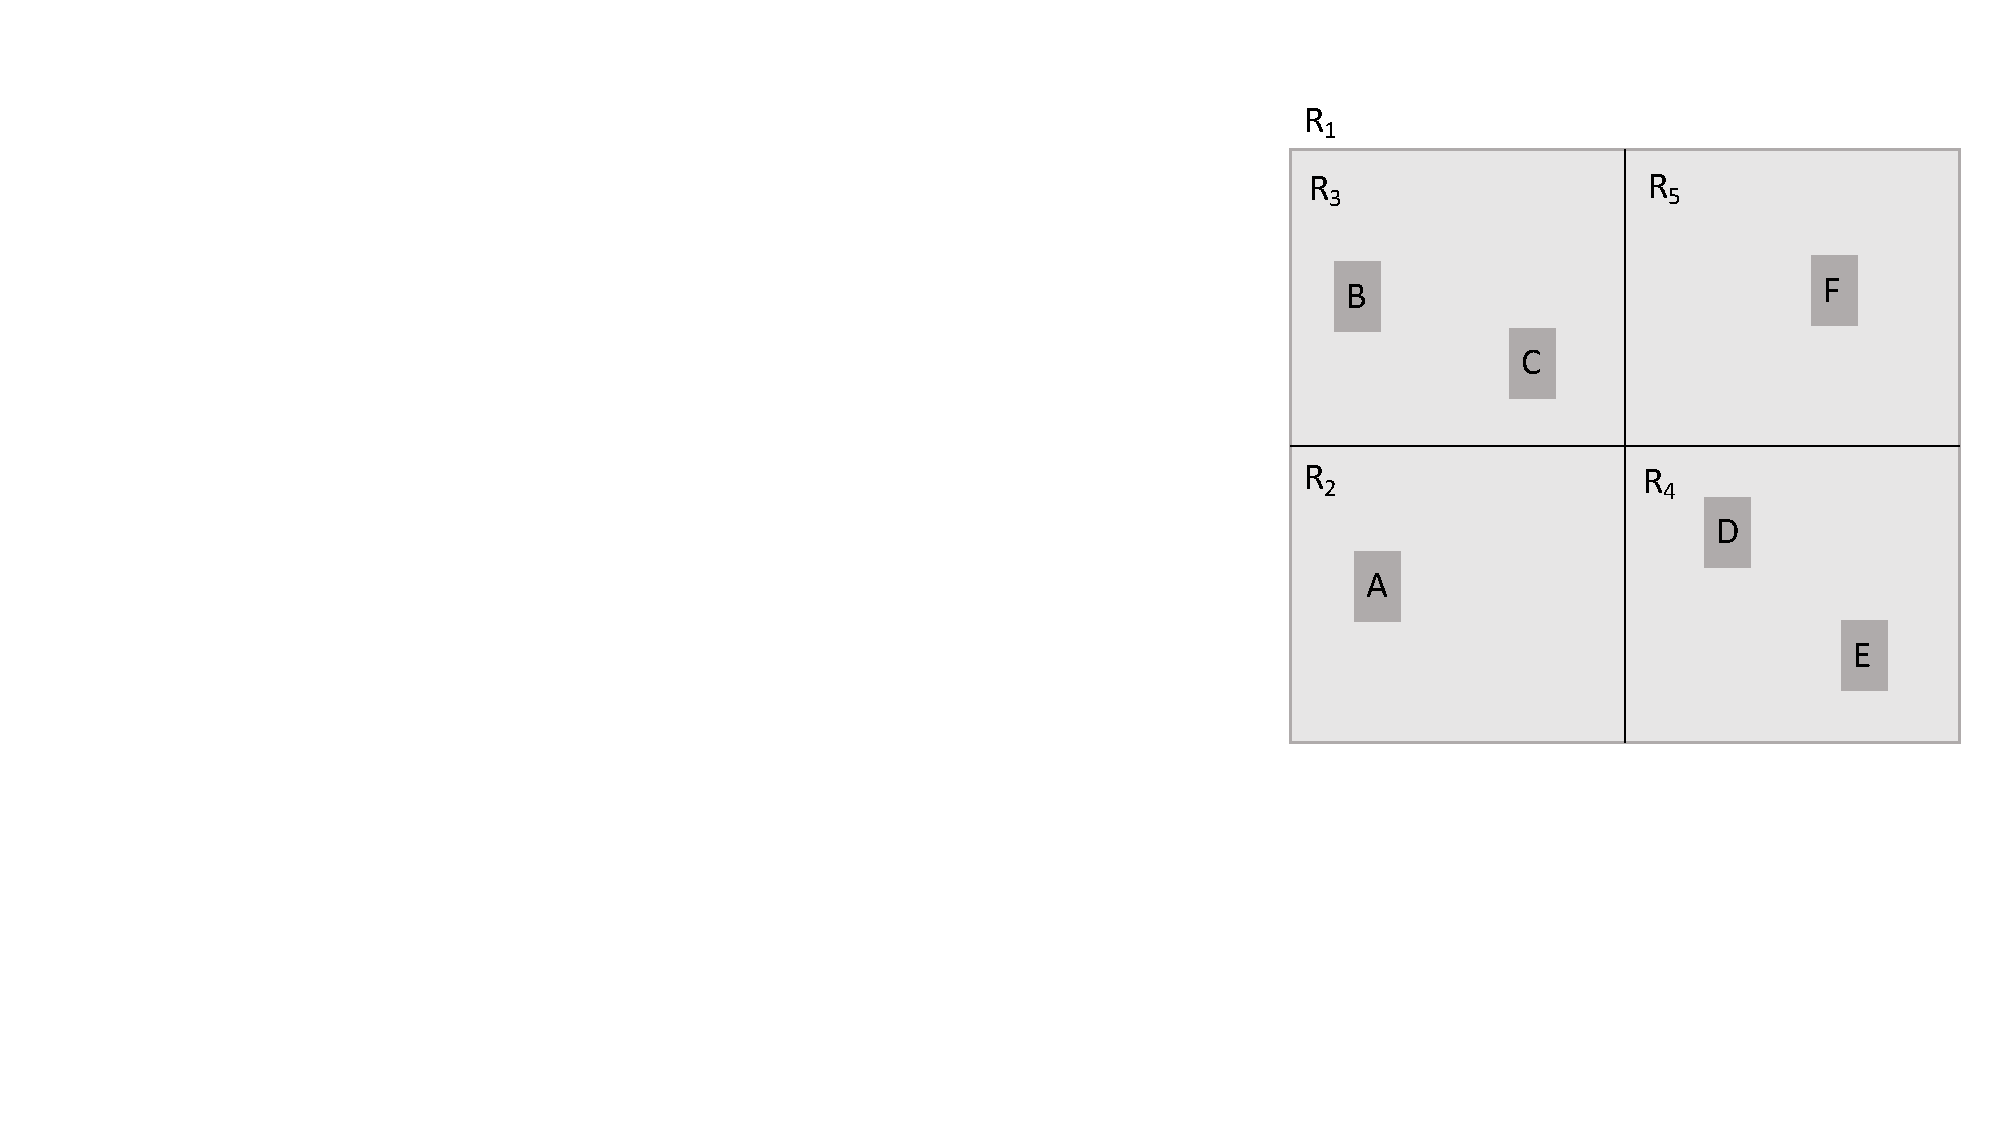
\includegraphics[width=\textwidth]{figures/RSMTree_space.pdf}
         \caption{RSM-Tree space structure}
     \end{subfigure}
        \caption{RSM-Tree}
        \label{fig:RSMTree}
\end{figure}

\noindent
The nodes in the RSM-tree are structured as shown in Figure \ref{fig:nodeRSM}. The first value is the Z-order value calculated from the object's minimum bounding rectangle (MBR), while the MBR is the rectangle containing the object. The last element, \emph{pointer}, points to either an intermediate node's child nodes or an object identifier. The calculation of the Z-order values is explained in Section \ref{sect:zordering}. 

\begin{figure}[ht]
    \centering
    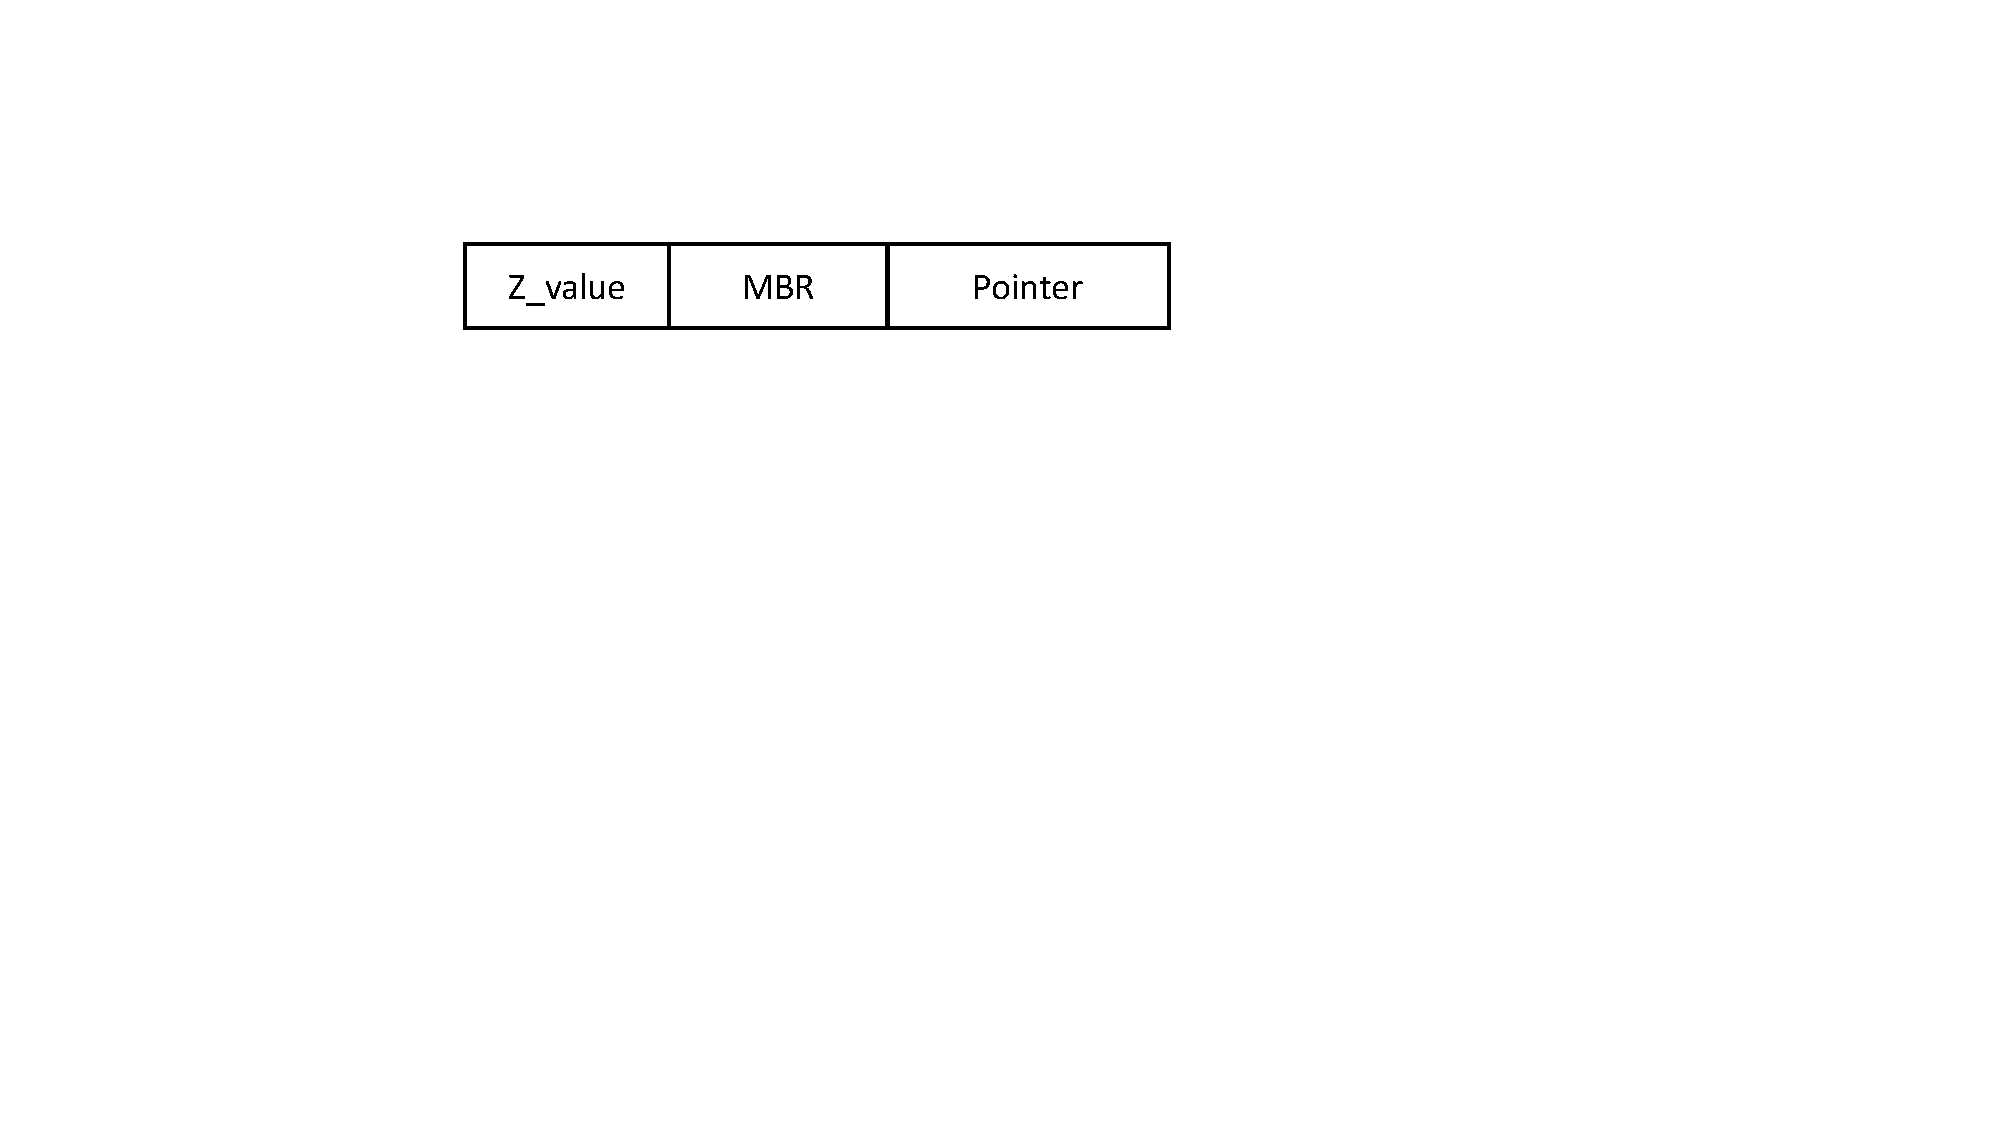
\includegraphics[scale=0.5]{figures/node_RSM.pdf}
    \caption{RSM-Tree Node structure}
    \label{fig:nodeRSM}
\end{figure}

\section{Space-Filling Curve}
\label{sect:ordering}
The use of a space-filling curve when creating the RSM-tree is crucial in order to sequentially order the objects in level $C_0$. As Z-ordering is simpler to implement, as well as being less costly, it will be the implemented technique. This is also because it has proven to perform well with a low number of dimensions\cite{IrregularSpace}, which will be the case when inserting test data in a future implementation. When further developing the RSM-tree, it is also possible to implement the Hilbert curve ordering technique, but this will not be a priority during the first implementation. 

\subsection{Z-ordering}
\label{sect:zordering}
To calculate the Z-order value of each object, the $x$ and $y$ coordinates of each object's MBR are found. These coordinates can be chosen as the outer corner of a rectangle or as the rectangle's center. In this design solution, the coordinates will be calculated from the center. These coordinates will then be represented as their binary value. In order to calculate the binary representation of the two coordinates together, their individual values are interleaved. Interleaving is done by extending $x$ and $y$ of length $n$ to length $2n$, where each value from $x$ is put in odd positions and each value from $y$ is put in even positions\cite{interleave}. This can also be done in an opposite manner. An example of this process is shown in Figure \ref{fig:bitInterleaving}, inspired by \cite{zorder_figure}. The space is considered for integers between 0 and 7, but only showing the first quadrant in Figure \ref{fig:zspace}. The interleaving process of this first quadrant is demonstrated in Figure \ref{fig:zinterleave}, where the $x$ coordinate is set at even positions while the $y$ coordinate is set at odd positions. By finding the binary representation of a position, we can use this information to compare objects when ordering them. 

\begin{figure}[ht]
     \centering
     \begin{subfigure}{0.45\textwidth}
         \centering
         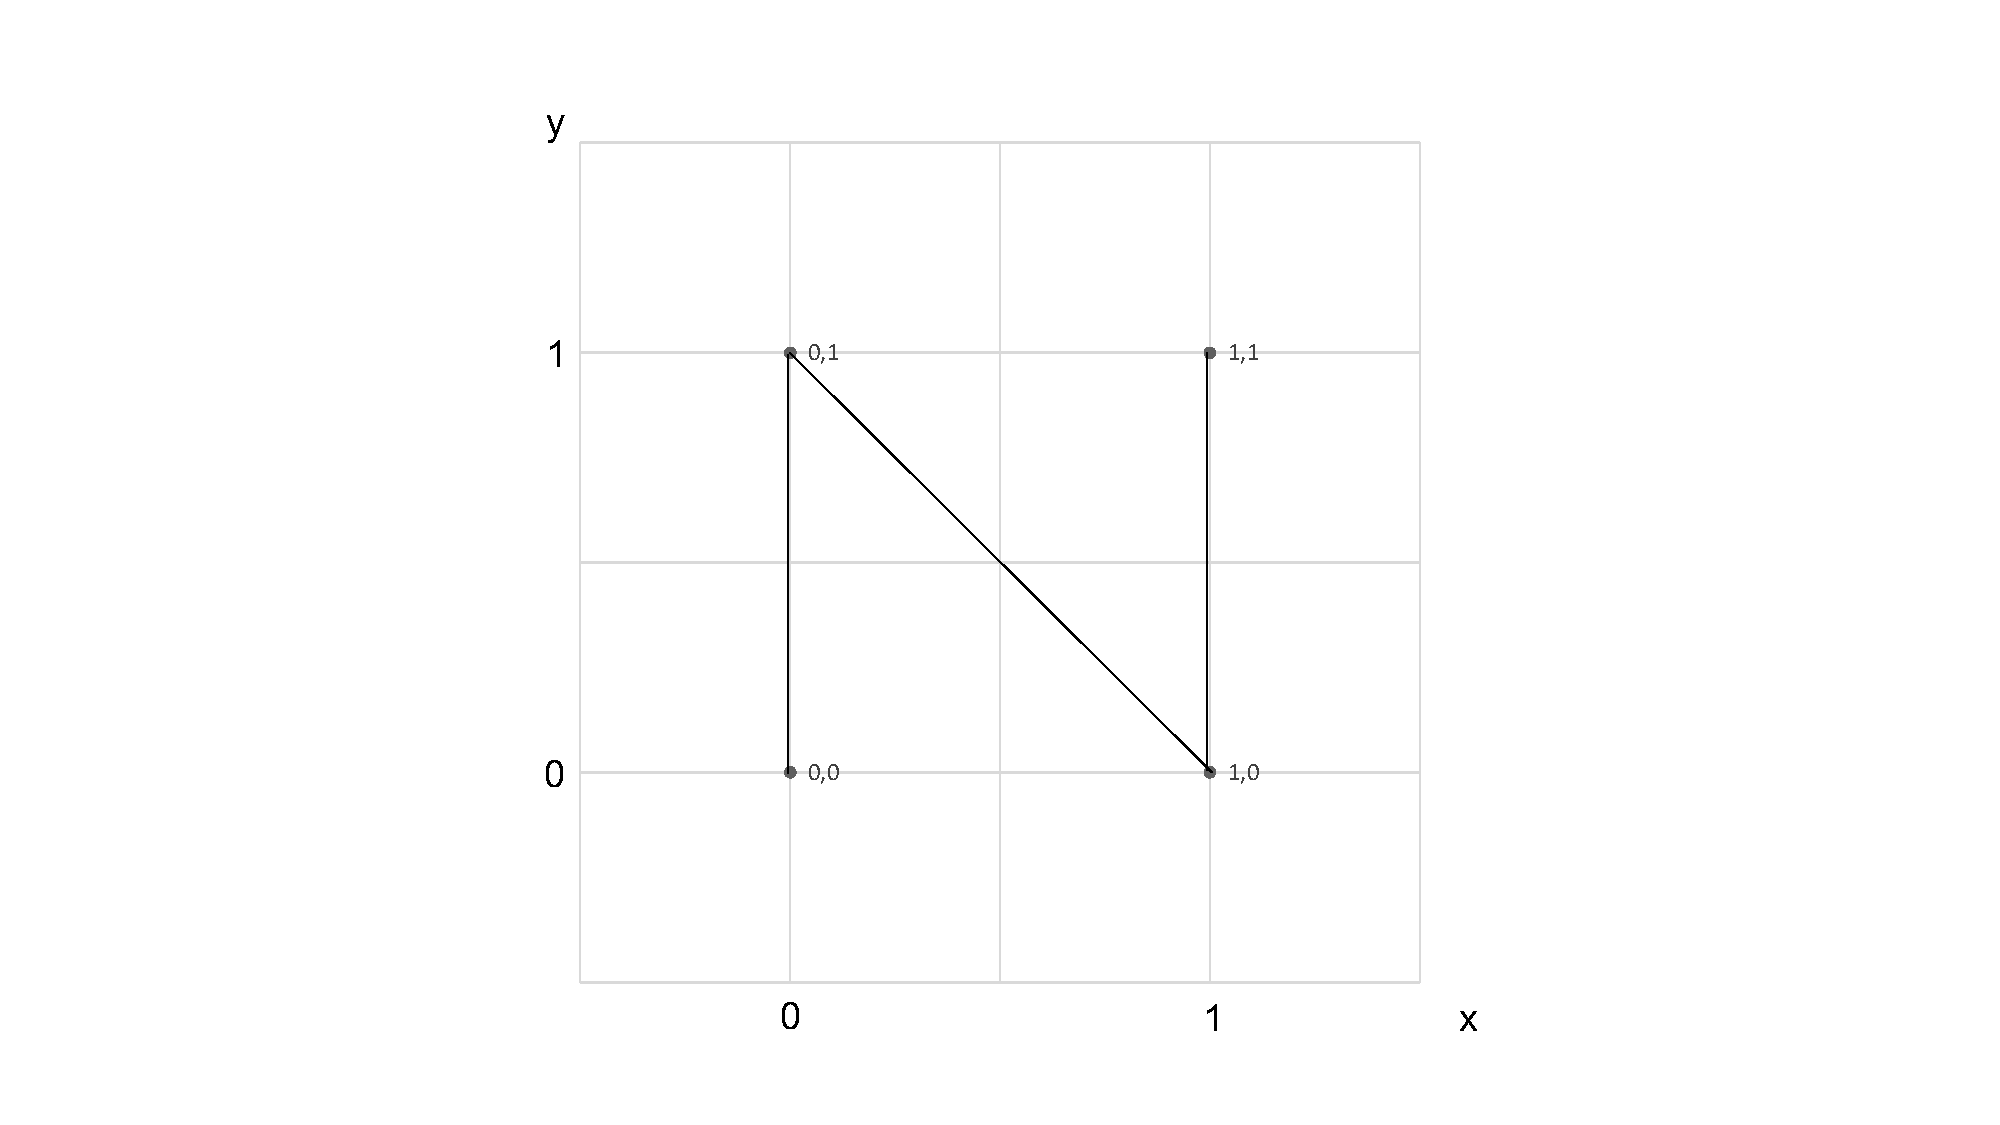
\includegraphics[width=\textwidth]{figures/zorder_process_graph.pdf}
         \caption{Z-order mapping in space}
         \label{fig:zspace}
     \end{subfigure}
     \hfill
      \begin{subfigure}{0.45\textwidth}
     \centering
     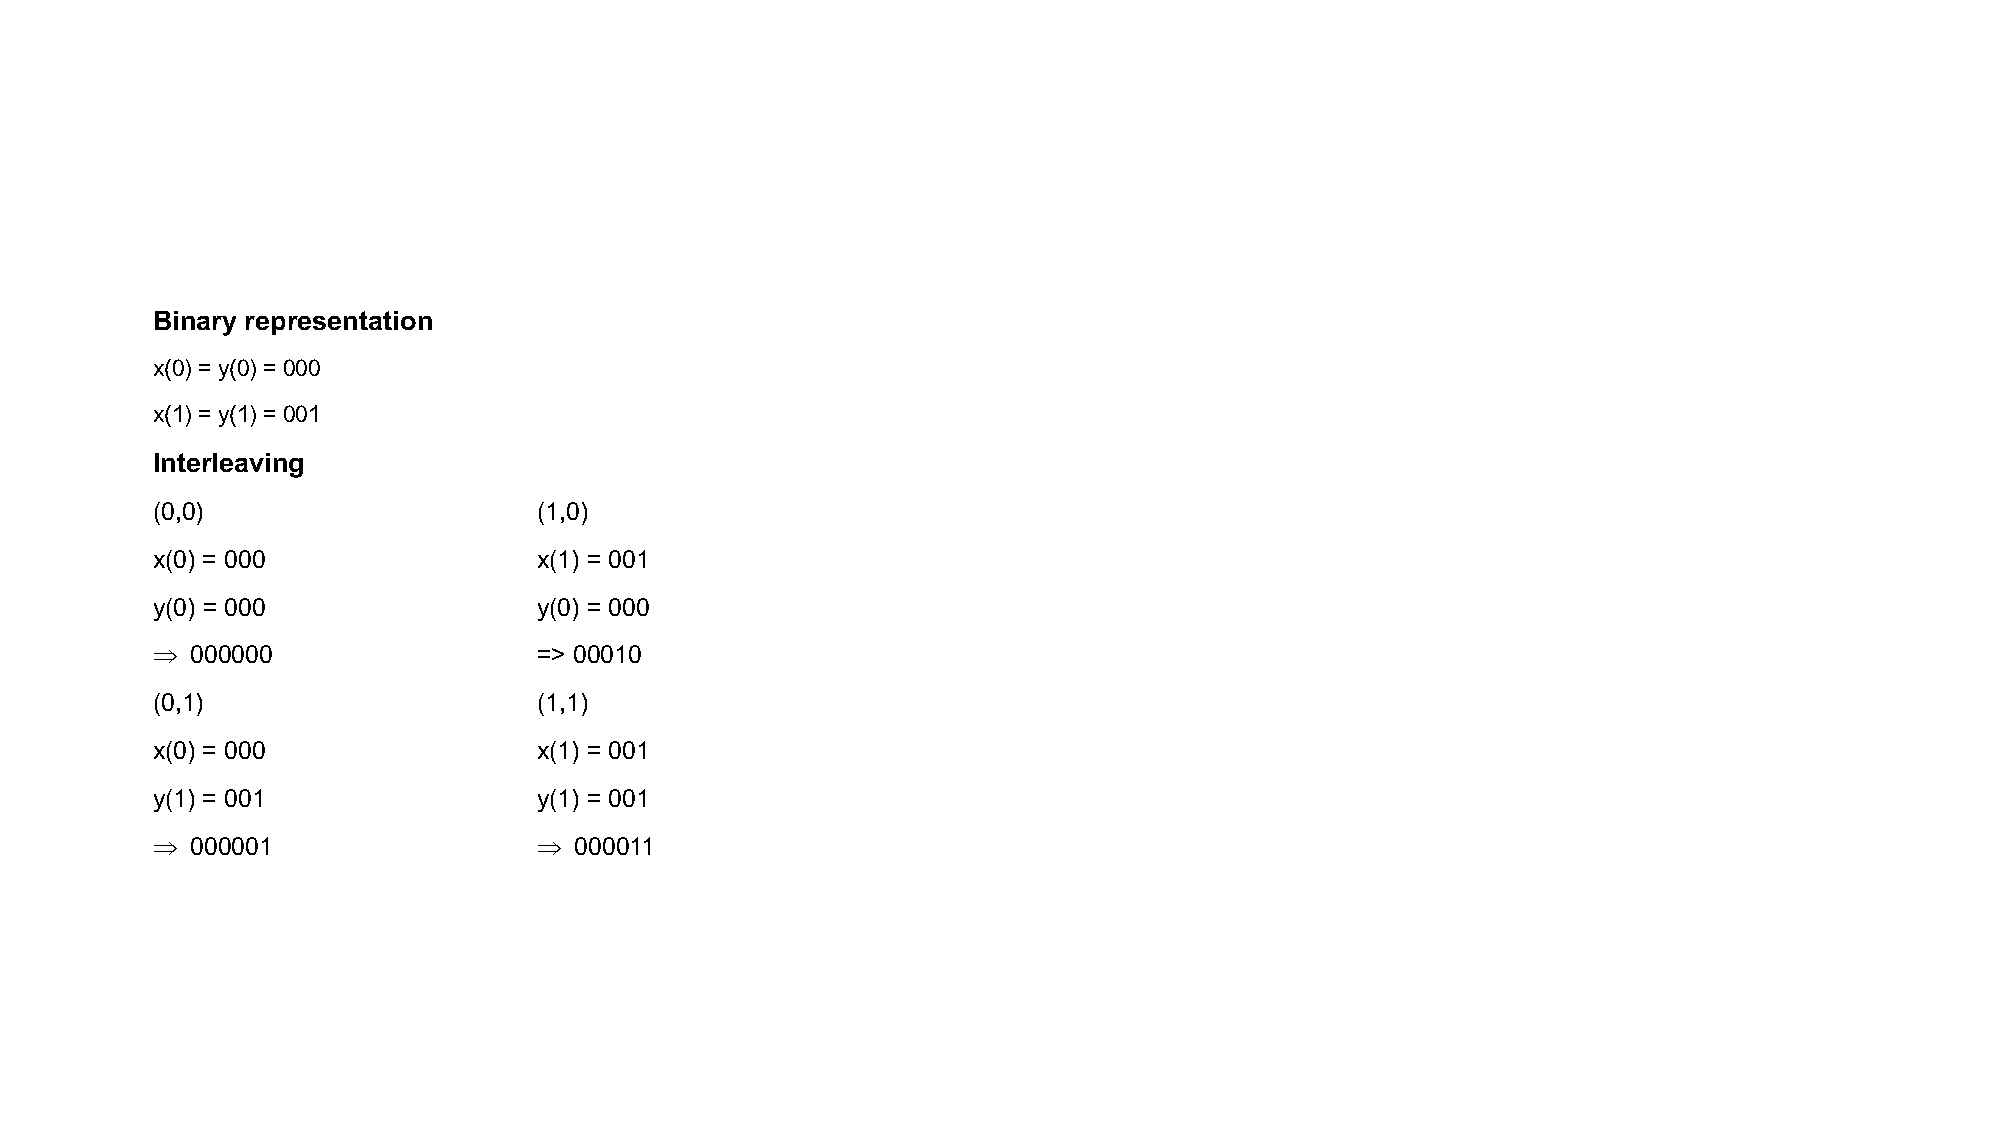
\includegraphics[width=\textwidth]{figures/zorder_process_interleaving.pdf}
     \caption{Interleaving process}
     \label{fig:zinterleave}
     \end{subfigure}
    \hfill
    \caption{Z-order calculation process}
    \label{fig:bitInterleaving}
\end{figure}

\section{Merging}
\label{sect:RSM-Merging}
The merging technique for the RSM-tree is based on both construction of R-trees from scratch, in addition to using bulk-insertion into existing trees. The initial design solution is made up of three levels that each have some important characteristics. 

\subsection{Level $C_0$: In-memory component}
The in-memory component consists of single objects, ordered by the Z-order value of the center of each object's MBR. As in the regular LSM-tree, objects are sent to the lower level, $C_1$, when the total number of objects reach a certain threshold. 

\subsection{Level $C_1$: Upper-level storage component}
In an ideal solution, all elements coming from $C_0$ would be indexed in the same R-tree. But, as the trees in $C_1$ are constructed to be bulk-loaded into the main R-tree in level $C_2$, there are some considerations that need to be discussed. One important factor is the distribution of the data. If we were to construct R-trees based on their location in space (e.g., divide the space into the four squares given in Figure \ref{fig:RSMTree}), we could end up with having to restructure the main R-tree in $C_2$ if the data is skewed. This is due to the fact that we cannot insert R-trees into the same position in the main R-tree without requiring restructuring. This entails node splitting when overflow occurs, which in turn will lead to uneven depths in the different nodes, which leads to restructuring of the whole tree. This is due to the constraint that all leaf nodes must be at the same level of the tree. Another aspect is the area in space covered by each R-tree in $C_1$. If we simply create an R-tree from all objects coming from $C_0$, we could end up with intermediate nodes that cover a lot of empty space. This is because the objects might not be spatially close to each other. When these R-trees are bulk-inserted into the main R-tree, there is a higher chance for overlapping MBR's in intermediate nodes, as they each might cover a large area. \newline

\noindent
One way of handling these issues can be to use seeded clustering\cite{SeededClustering} and to look for outliers. By maintaining a clustering scheme, based on the top $k$ levels of the main R-tree, we can adjust the clustering to the data distribution. To implement this, the RSM-tree will have a seeded R-tree stored in $C_1$, which will be updated at an evenly rate. The data that comes from $C_0$ will then be assigned to clusters, and an R-tree per cluster will be created. By doing this, the main R-tree will most likely avoid too many overlapping MBR's in intermediate nodes, in addition to reducing the amount of node splits. If there are any outliers, these will be inserted into the main R-tree one-by-one. The construction of the R-trees in $C_1$ will follow the structure of the general R-tree proposed by Guttman\cite{r-tree}. If time allows, the Sort-Tile-Recursive packing method\cite{STR} might also be implemented as all objects for the R-trees are known before the construction.

\subsection{Level $C_2$: Lower-level storage component}
In the lowest level, $C_2$, the main R-tree will be stored. The R-tree is dynamically updated by bulk-insertions from $C_1$. As the trees coming from the level above are clustered according to the top $k$ levels of the main tree, we reduce the need for node splits. If node underflow should occur however, it is handled in the same way as described by bulk-insertion by seeded clustering\cite{SeededClustering}. If the incoming tree suffers from underflow, the elements in the incoming tree is reinserted at the target node in the main tree. Another important aspect is the repacking method, which is done if the insertion creates many overlapping entries. If a node overflows, the quadratic split method\cite{r-tree} is used. An important part of using seeded clustering is to find out how often a seeded tree should be generated and sent to level $C_1$. This is something that needs to be tested during the implementation, as generating it too often will use unnecessary resources, while if not updated often enough will lead to bad distribution for the incoming R-trees. 

\subsection{Merge policies}
As the goal for the RSM-tree is to be write-optimized, the main merge policy used is \emph{Lazy Leveling}\cite{Dostoevsky}. By having most of the merge performed at the lowest level, we can take advantage of having a higher write-throughput as well as maintaining adequate lookup and storage costs, as explained in Section \ref{Dostoevsky}. In the first implementation, the RSM-tree will consist of three levels, where the lowest level uses the leveling merge policy, while the second level uses the tiering merge policy. If time allows, it would be interesting to implement different combinations of the two merge policies, by using the implementation in \emph{Fluid LSM-trees}.  


\section{Insertion, Updates, Deletions}
Insertion, updates and deletions will be conducted in a similar manner as in the traditional LSM-tree. When an entry is inserted, an MBR is created for the object as well as calculating its Z-order value. This element is then inserted into $C_0$, in the correct position according to its Z-order value. The rest of the insertion process will be as described in Section \ref{sect:RSM-Merging}. Deletions are done by either deleting the object directly, if it is present in $C_0$, or creating a deletion block which is sent through the levels. A deletion block will consist of the same elements as a regular node, but will have an additional entry indicating that it is meant to be deleted. This is then used in $C_1$ and $C_2$ to search for overlapping MBR's to identify the object to delete. Updates are handled by first deleting an entry, followed by inserting a new one. 


\section{Evaluation}
In order to evaluate the RSM-tree, there are different metrics that need to be adjusted and compared. The main metrics and parameters that will be looked at are:\newline

\noindent
\textbf{Write Throughput} is maybe the most important metric to test for the RSM-tree, as it is the ultimate goal that the write throughput is higher than in the general R-tree. This will be tested with different data distributions to see if the RSM-tree favours skew or uniform data. \newline

\noindent
\textbf{I/O operations} is another important measure to measure write and read amplification. For read amplification this will be tested by executing queries, as it is important that the RSM-tree maintains a certain query performance. The write amplification will be measured during insertion, by counting number of blocks written to, including its final storage block in the lowest level. \newline

\noindent
\textbf{Tree fanout} should be looked at with regard to performance. This is decided by setting the maximum number of entries a node can contain. It is important to find a setting so that the tree is not too deep, which adds to number of paths accessed during a search, and not too wide, which will cause a search operation to sequentially search most of the entries, as there are many entries in each node. \newline

\noindent
\textbf{Seeded clustering} should be tested with different parameters. This entails both how often the seeded tree should be created from the main R-tree, and how many levels the seeded tree should be made of. \newline

\noindent
\textbf{Component size} of the different levels $C_0$, $C_1$ and $C_2$ needs to be tested. If the component sizes are too big, the entries to be merged may be many, which in turn can make the process slower. If the components are too small however, the merge procedure might be executed more often than needed. The sizes will also impact the search performance, both because the search might have to run through many levels, and because the search might have to search through many trees in $C_1$.\newline

\noindent
After the most efficient parameters are found for the node size, the seeded tree and the component sizes, the performance of the RSM-tree will be compared to the general R-tree create by Guttman\cite{r-tree}. 

\subsection{Test Data}
There are many aspects to take into consideration when using test data to eventually evaluate the implementation of the design solution. The first is that the results should be unbiased and that the test data should consist of different distributions to uncover how the design performs in different situations. Second, it is beneficial to use both synthetic data and real-world data for testing. Synthetic data is adjustable, and we can therefore create both skew and uniform distributions. This is not as easily manufactured when using real-world data. It is however still important to also test the design solution with a dataset from the real world, to show how it performs with neutral data. With neutral data, we mean data that has not been created for a specific outcome, and is a way to show that results given are not only generated by creating data that ensures positive numbers.\newline

\noindent
In order to ensure unbiased and varied data, different synthetic datasets should be created. These should included skewed, slightly-skewed and uniform data. The data should also be created with a different number of dimensions, as the space-filling curves are a large part of the design solution and can be highly impacted by the dimensionality. In addition, a real-world dataset should be included. An example of this could be either sensor data capturing weather conditions or device usage based on geographical locations. Lastly, an important aspect of the design solution is how well query performance is, as it is crucial that the RSM-tree is still able to handle queries, even though the goal is to increase write-performance. It is therefore important to have test data that is possible to query across dimensions and locations in space. 